\documentclass[border=4pt]{standalone}
\usepackage{amsmath,amssymb,tikz}\usetikzlibrary{arrows.meta}
\definecolor{figB}{RGB}{31,90,166}\definecolor{figR}{RGB}{176,48,48}\definecolor{figG}{RGB}{46,125,50}\definecolor{figO}{RGB}{214,120,20}
% T(z1,z2,z3) = (4 z2, 0, 5 z3), drawn over R: null T = z1-axis, range T = z1z3-plane;
% null T^3 = z1z2-plane, range T^3 = z3-axis.
\begin{document}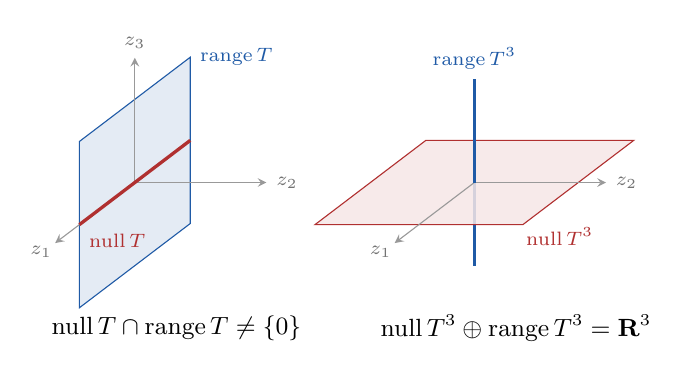
\begin{tikzpicture}[scale=0.88,>={Stealth[length=1.8mm]},x={(-0.5cm,-0.38cm)},y={(1cm,0cm)},z={(0cm,1cm)}]
\begin{scope}
\fill[figB!12] (-1.6,0,-1.2)--(1.6,0,-1.2)--(1.6,0,1.2)--(-1.6,0,1.2)--cycle;
\draw[figB] (-1.6,0,-1.2)--(1.6,0,-1.2)--(1.6,0,1.2)--(-1.6,0,1.2)--cycle;
\draw[black!40,thin,-stealth] (0,0,0)--(2.3,0,0) node[below left,font=\scriptsize,black!55,inner sep=1pt]{$z_1$};
\draw[black!40,thin,-stealth] (0,0,0)--(0,1.9,0) node[right,font=\scriptsize,black!55]{$z_2$};
\draw[black!40,thin,-stealth] (0,0,0)--(0,0,1.8) node[above,font=\scriptsize,black!55]{$z_3$};
\draw[very thick,figR] (-1.6,0,0)--(1.6,0,0);
\node[font=\scriptsize,figB,anchor=west] at (-1.6,0,1.2) {$\operatorname{range}T$};
\node[font=\scriptsize,figR,anchor=north west] at (1.6,0,0) {$\operatorname{null}T$};
\node[font=\small,align=center] at (0,0.6,-2.1) {$\operatorname{null}T\cap\operatorname{range}T\ne\{0\}$};
\end{scope}
\begin{scope}[xshift=4.9cm]
\draw[very thick,figB] (0,0,-1.2)--(0,0,0);
\fill[figR!12,opacity=0.85] (-1.6,-1.5,0)--(1.6,-1.5,0)--(1.6,1.5,0)--(-1.6,1.5,0)--cycle;
\draw[figR] (-1.6,-1.5,0)--(1.6,-1.5,0)--(1.6,1.5,0)--(-1.6,1.5,0)--cycle;
\draw[black!40,thin,-stealth] (0,0,0)--(2.3,0,0) node[below left,font=\scriptsize,black!55,inner sep=1pt]{$z_1$};
\draw[black!40,thin,-stealth] (0,0,0)--(0,1.9,0) node[right,font=\scriptsize,black!55]{$z_2$};
\draw[very thick,figB] (0,0,0)--(0,0,1.5);
\node[font=\scriptsize,figB,anchor=south] at (0,0,1.5) {$\operatorname{range}T^3$};
\node[font=\scriptsize,figR,anchor=north west,inner sep=1pt] at (1.6,1.5,0) {$\operatorname{null}T^3$};
\node[font=\small] at (0,0.6,-2.1) {$\operatorname{null}T^3\oplus\operatorname{range}T^3=\mathbf{R}^3$};
\end{scope}
\end{tikzpicture}\end{document}
